\documentclass[11pt]{beamer}

\usetheme[progressbar=frametitle]{metropolis}
\usepackage{appendixnumberbeamer}
\usepackage{FiraSans}
\usepackage{textcomp} %% put this in your preamble
\usepackage{graphicx} 
\usepackage{booktabs}
\usepackage[scale=2]{ccicons}
\usepackage{adjustbox}
\usepackage{soul}
\usepackage{caption}
	\captionsetup[figure]{	labelformat=empty, 
					font=scriptsize,
					labelfont=scriptsize, 
					justification=raggedleft}

\usepackage{pgfplots}
\usepgfplotslibrary{dateplot}



\usepackage{xspace}
\newcommand{\themename}{\textbf{\textsc{metropolis}}\xspace}

\title{The ecology of summer prescribed fire regimes in the Northern Great Plains }
\subtitle{Meet the Researcher \\Tallgrass Prairie \& Oak Savanna Fire Science Exchange \vspace{-1em}}
\date{}
\author[shortname]{\textbf{Devan Allen McGranahan}  }
\institute[shortinst]{USDA Agricultural Research Service: Miles City, MT \\
	\vskip %\vspace{0.5em}
All data from the paper: \\
% \vspace{0.5em}
McGranahan \& Angerer (2025) \emph{Evaluating an attempt to restore summer fire in the Northern Great Plains}. Environmental Management 75:1656–64 \\
All photo credit to the author }

\newcommand\blfootnotetext[1]{%
	\begingroup
	\renewcommand\thefootnote{}\footnote{#1}%
	\addtocounter{footnote}{-1}%
	\endgroup
}


\begin{document}

\maketitle

\begin{frame}{Briefing}
%	\vspace{-3em}	
	\begin{columns}
		
		\begin{column}{0.4\textwidth}
			\begin{itemize} 
				\item Fire regimes \& R\textsubscript{x} fire management
					\item[]
				\item Ways to measure, describe fire
				\item[]
				\item Feasibility of summer fires
				\item[]

				%	\item Relative severity of wildfire \& R\textsubscript{x} burns
				
			\end{itemize}
			
		\end{column}
		\begin{column}{0.6\textwidth}  
			\begin{center}
				\begin{figure}
					\includegraphics[width=1\linewidth]{figs/BriefingCircle} 
					
				\end{figure}
			\end{center}
		\end{column}
	\end{columns}
\end{frame}

\begin{frame}{The Western fire regime concept\footnote{McGranahan \& Wonkka (2021) \emph{Ecology of Fire-Dependent Ecosystems} } } 
	\begin{center}
		\begin{figure}
			\includegraphics[width=1\linewidth]{figs/FireRegimeNAPC} 
		
		\end{figure}
	\end{center}
\end{frame}

\section{Measuring wildland fire}

\begin{frame}{Direct measurements of fire behavior}
			\begin{itemize}
		\item \emph{Temperature}\textemdash Flames, soil heat exposure
		\item \emph{Rate of spread}\textemdash 2-D thermocouple array
		\item \emph{Fireline intensity}\textemdash rate of energy release
	\end{itemize}
	\begin{columns}
		\begin{column}{0.5\textwidth}
			\begin{center}
				\begin{figure}
					\includegraphics[width=1\linewidth]{figs/FireTree} 
					
				\end{figure}
			\end{center}
		\end{column}
		\begin{column}{0.5\textwidth}
			\begin{center}
				\begin{figure}
					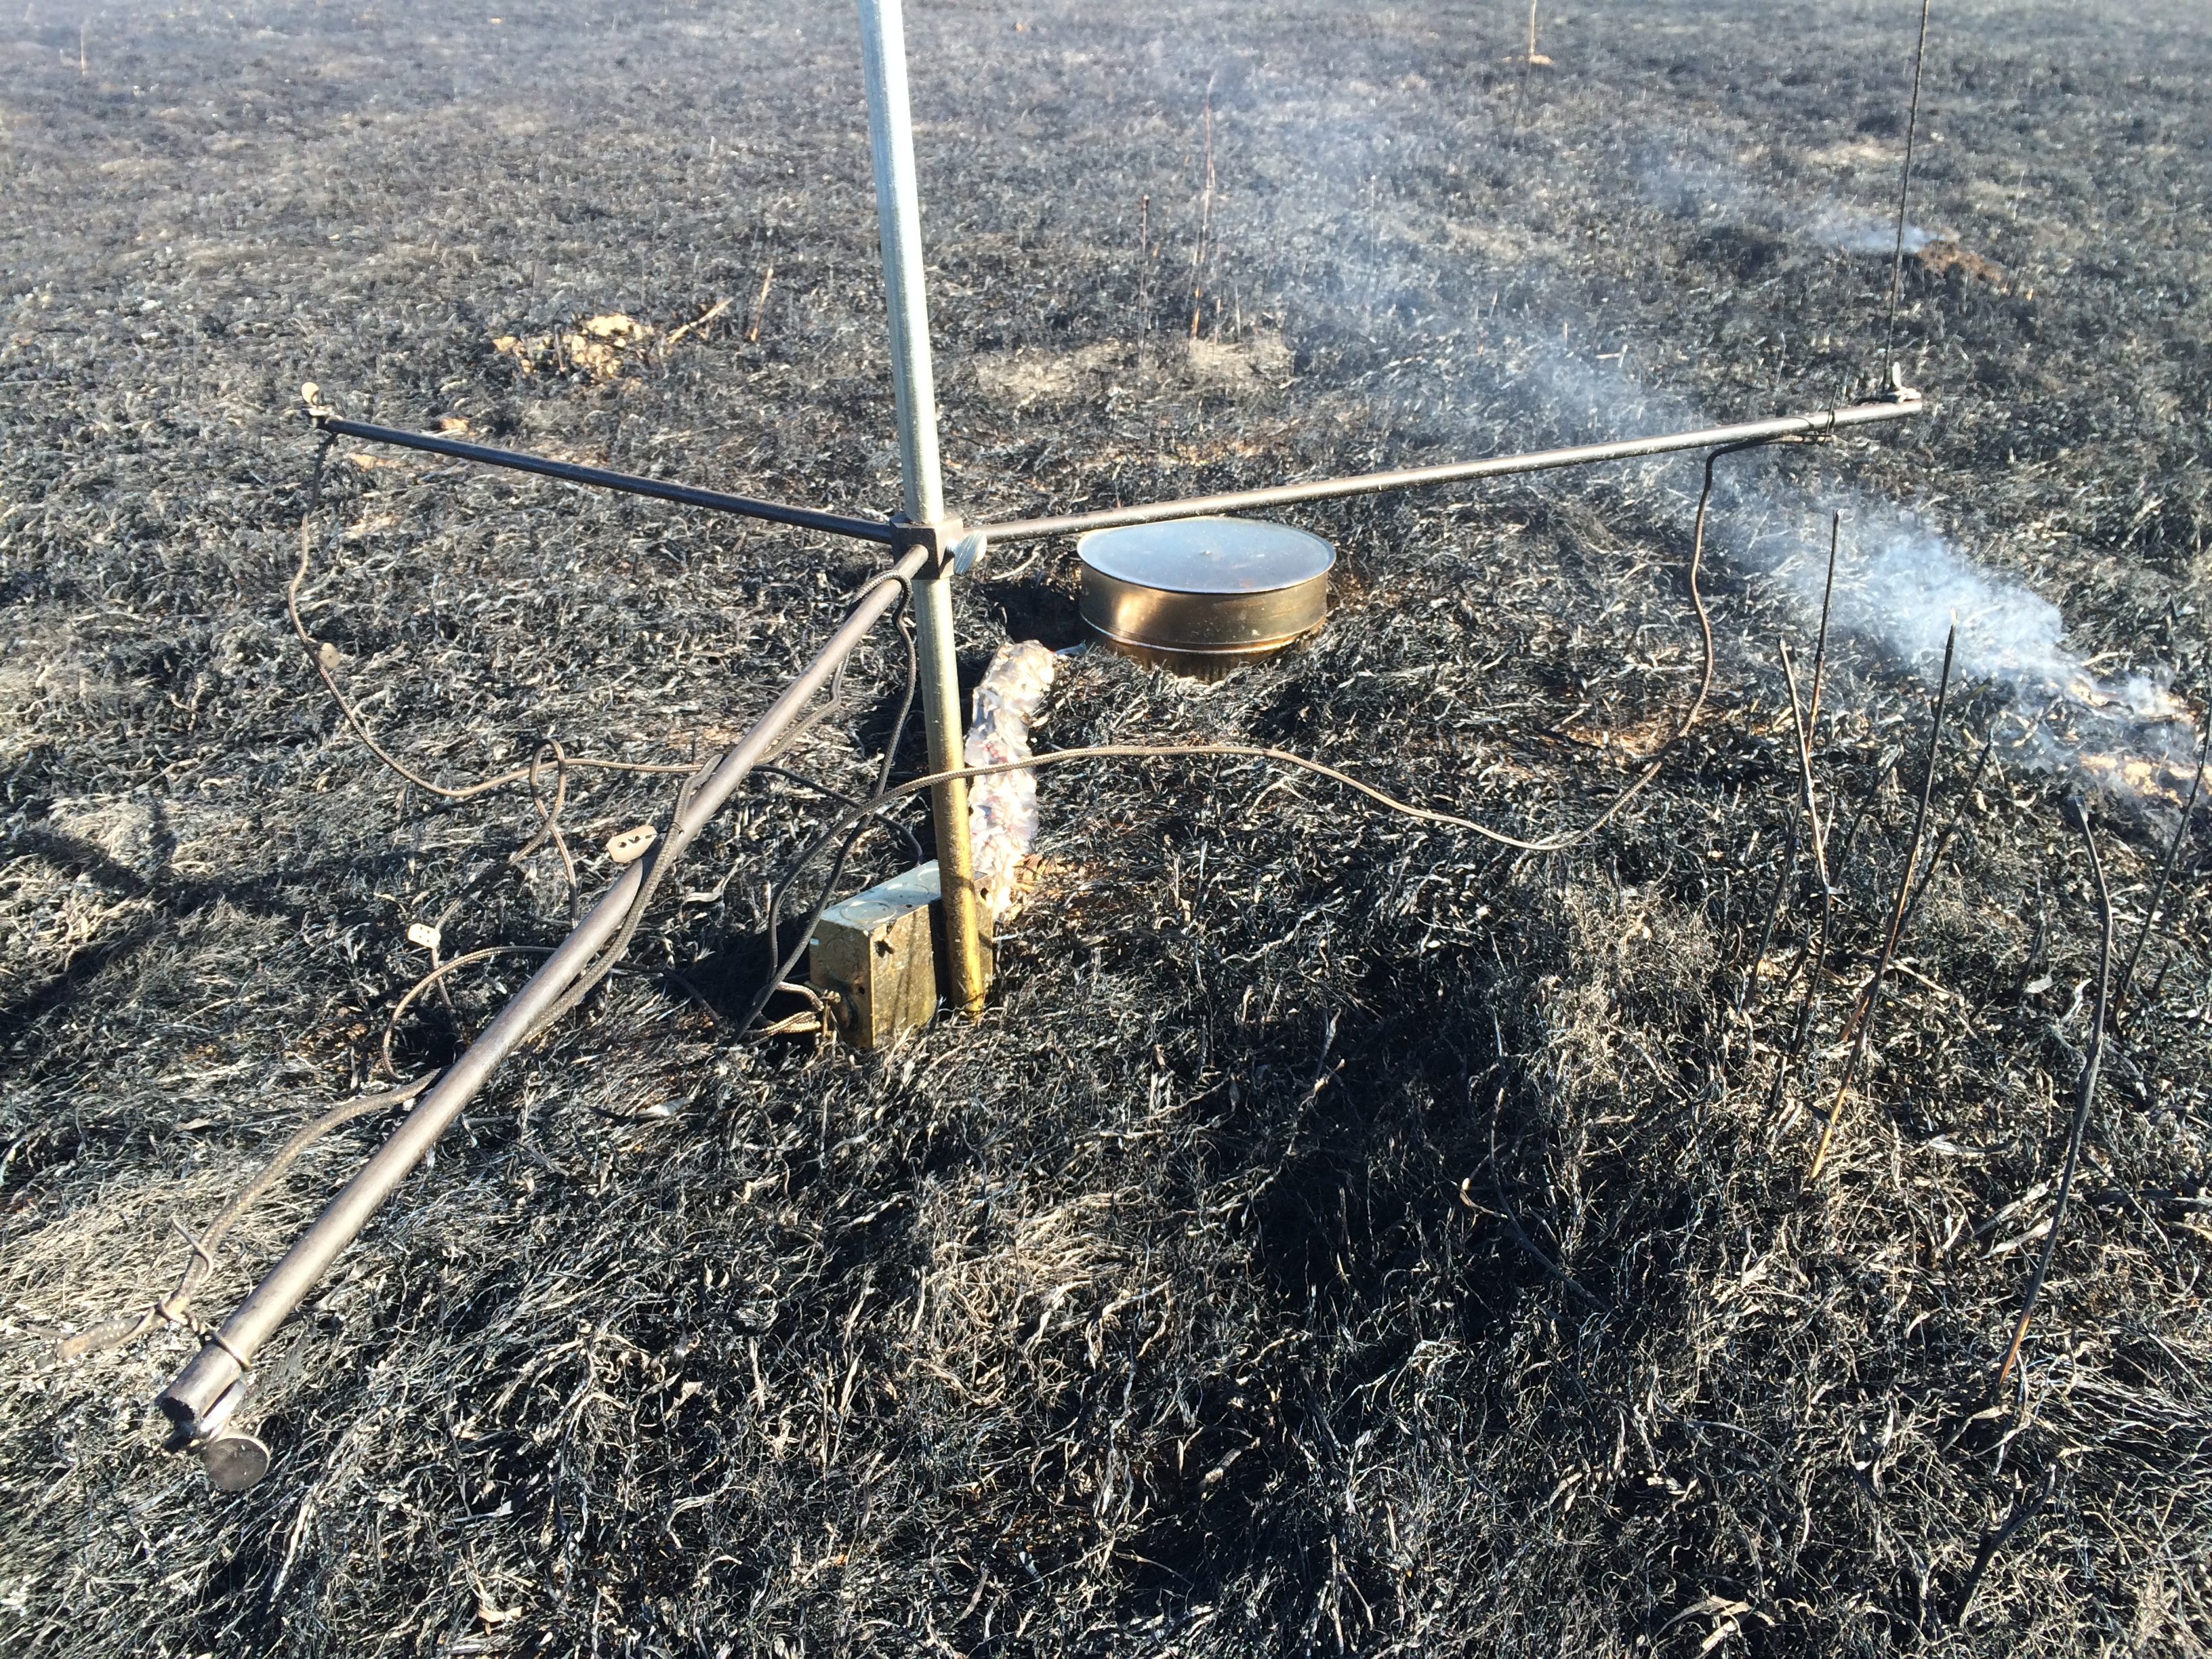
\includegraphics[width=1\linewidth]{figs/TCtree} 	
				\end{figure}
			\end{center}
		\end{column}
	\end{columns}
\centering
\alert{ Describe differences in \textbf{fire effects} by understanding variability in \textbf{how it burned}} 
\end{frame}

\begin{frame}{Satellite imagery informs burn severity}
	True-color images of a North Dakota wildfire from space
	\begin{center}
		\begin{figure}
			\includegraphics[width=1\linewidth]{../SatelliteFireSpread} 
		\end{figure}
	\end{center}
\end{frame}

\begin{frame}{Satellite imagery informs burn severity}
Comparing  multispectral imagery = Burn Severity
	\begin{center}
		\begin{figure}
			\includegraphics[width=1\linewidth]{../NBRexample} 
		\end{figure}
	\end{center}
\end{frame}

\begin{frame}{``Burn severity'' and ``fire behavior'' correlate pretty well}
	\begin{center}
						If burn severity works as proxy for fire behavior ...
		\begin{figure}
			\includegraphics[width=1\linewidth]{../dNBR_v_FB-1.png} 
		\end{figure}

				\alert{... managers might better understand variability in fire effects without collecting (much) data}
	\end{center}
\end{frame}

\section{Seasonality \& management}

\begin{frame}{For every season: Burn, burn, burn...}
	
	\begin{columns}
		\begin{column}{0.5\textwidth}
			\begin{itemize} 
				\item Conventionally: R\textsubscript{x} fire conducted primarily during dormant season
				\item[]
				\item Increased interest in burning during non-dormant season
				\item[]
				\begin{itemize}
					\item Awareness of pre-colonial fire regimes
					\item Diversify management
				\end{itemize}
				
			\end{itemize}
			
		\end{column}
		\begin{column}{0.5\textwidth}  
			\begin{center}
				\begin{figure}
					\includegraphics[width=1\linewidth]{figs/StreeterRxFire} 
					
				\end{figure}
			\end{center}
		\end{column}
	\end{columns}
% \alert{As with most fire regime parameters, \textbf{seasonality is a construct}}
\end{frame}

\begin{frame}{Case study: R\textsubscript{x} fire in the Northern Great Plains}
	\begin{center}
		\begin{figure}
			\includegraphics[width=1\linewidth]{figs/region_map-1.pdf} 
		\end{figure}
	\end{center}
\end{frame}

\begin{frame}{R\textsubscript{x} fire in the Northern Great Plains}
	\begin{center}
		\begin{figure}
			\includegraphics[width=1\linewidth]{figs/PBGmaps} 
		\end{figure}
	\end{center}
\end{frame}

\begin{frame}{Two-for-four in completing summer burns}

	\begin{center}
		\begin{figure}
			\includegraphics[width=0.9\linewidth]{figs/BarkerBurns-1} 
			\caption{Final burn map for southern study block}
		\end{figure}
	\end{center}
\end{frame}

\begin{frame}{Spring fire: What a difference a few days make! } 
	\begin{columns}
		\begin{column}{0.5\textwidth}
				\begin{center}
				\begin{figure}
					%\caption{5 May 2018}
					\includegraphics[width=0.9\linewidth]{figs/GoodBurn} 
				\end{figure}
			\end{center}
		\end{column}
		\begin{column}{0.5\textwidth}  
			\begin{center}
				\begin{figure}
					%\caption{16 May 2018}
					\includegraphics[width=1\linewidth]{figs/StreeterFire_17}  
				\end{figure}
			\end{center}
		\end{column}
	\end{columns}
\centering
\adjustbox{max height=\dimexpr\textheight-5.5cm\relax,
	max width=1\textwidth}{
	\begin{tabular}{ccc}
		\toprule
		5 May 2018 & \textbf{Date} & 16 May 2018 \\
		79 & \textbf{Air temp (F)} & 82 \\
		5.9 & \textbf{Wind (m s\textsuperscript{-1})} & 2.4 \\
		22 & \textbf{min RH (\%)} & 24 \\
		37 & \textbf{Dew Point (F)} & 46 \\\bottomrule
	\end{tabular}
}
\end{frame}

\begin{frame}{Spring fire: Green fuels reduce burn severity}
	
	\begin{columns}
		\begin{column}{0.6\textwidth}  
			%\begin{center}
				\begin{figure}
					\includegraphics[width=1\linewidth]{figs/spring_burn_severity-1} 
					
				\end{figure}
			% \end{center}
		\end{column}
		\begin{column}{0.4\textwidth}
	\begin{figure}
	\includegraphics[trim=50cm 0cm 0cm 0cm, clip, 
					width=1\linewidth]{figs/WonkkaFlipped} 
	
\end{figure}
			
		\end{column}
		
	\end{columns}
\end{frame}

\begin{frame}{Summer fire: Fuels are much greener! }
	
	\begin{columns}
		\begin{column}{0.6\textwidth}  
			%\begin{center}
			\begin{figure}
				\includegraphics[width=1\linewidth]{figs/spring_burn_severity-1} 
				
			\end{figure}
			% \end{center}
		\end{column}
		\begin{column}{0.4\textwidth}
			\begin{figure}
				\includegraphics[%trim=50cm 0cm 0cm 0cm, clip, 
								width=1\linewidth]{figs/seasonal_ndvi-1} 
			\end{figure}
		\end{column}
	\end{columns}
\end{frame}

\begin{frame}{Summer fire: High severity possible even with green fuels }
	
	\begin{columns}
		\begin{column}{0.99\textwidth}  
			%\begin{center}
			\begin{figure}
				\includegraphics[width=1\linewidth]{figs/all_burn_severity-1} 
				
			\end{figure}
			% \end{center}
		\end{column}
		\begin{column}{0.01\textwidth}
			
		\end{column}
	\end{columns}
\end{frame}

\begin{frame}{Summer fire: Role of fire weather }
\emph{The terrible, humid, green, no-good day}

	\begin{columns}
		\begin{column}{0.65\textwidth}
			
			\begin{itemize} 
				\item[]\alert{13 August 2018}
				\item Forecast called for $<~40\%$ RH by noon, but...
				\begin{itemize}
					\item 54\% at 1200
					\item 50\% at 1500
				\end{itemize}
				\item[]
				\item Moisture constraints on ignition and spread
				\begin{itemize}
					\item Transpiration by green plants
					\item Humid air resists heating, lift
				\end{itemize}
				\item[]
				\item[] \alert{What \emph{normal} can managers expect?} 
				
			\end{itemize}
			
		\end{column}
		\begin{column}{0.4\textwidth}  
			\begin{center}
				\begin{figure}
					\includegraphics[width=0.9\linewidth]{figs/TorreGreenFuel} 
					
				\end{figure}
			\end{center}
		\end{column}
	\end{columns}
\end{frame}


\begin{frame}{42 years of fuel \& precipitation history}
	
\begin{itemize} 
	\item Successful burn seasons were within historical norms
	\item Summers without fire were historical anomalies
\end{itemize}

			\begin{center}
			\begin{figure}
				\includegraphics[width=1\linewidth]{figs/green_trends-1} 
				
			\end{figure}
			\end{center}

\end{frame}

\begin{frame}{42 years of \textbf{change} in fuel \& weather }
	
	\begin{itemize} 
	\item Greener but less humid springs?
	\item Less windy summers??
\end{itemize}
	
	\begin{center}
		\begin{figure}
			\includegraphics[width=1\linewidth]{figs/historical_phenology-1} 
			
		\end{figure}
	\end{center}
	
\end{frame}

\begin{frame}{Main take-aways}
	%	\vspace{-3em}	
	\begin{columns}
		
		\begin{column}{0.6\textwidth}
			\begin{itemize} 
				\item Summer burns ought to be possible more often than not
				\item[]
				\item Potential no-go thresholds, \emph{but likely site-specific}
				\item[]  Examples from these data:
					\begin{itemize} 
					\item NDVI $>$ 0.55-0.6?
					\item $>$ ~275 mm rain by Aug 1?
					\end{itemize}
				\item[]
				\item  Little evidence conditions are substantially changing
	
			\end{itemize}
			
		\end{column}
		\begin{column}{0.4\textwidth}  
			\begin{center}
				\begin{figure}
					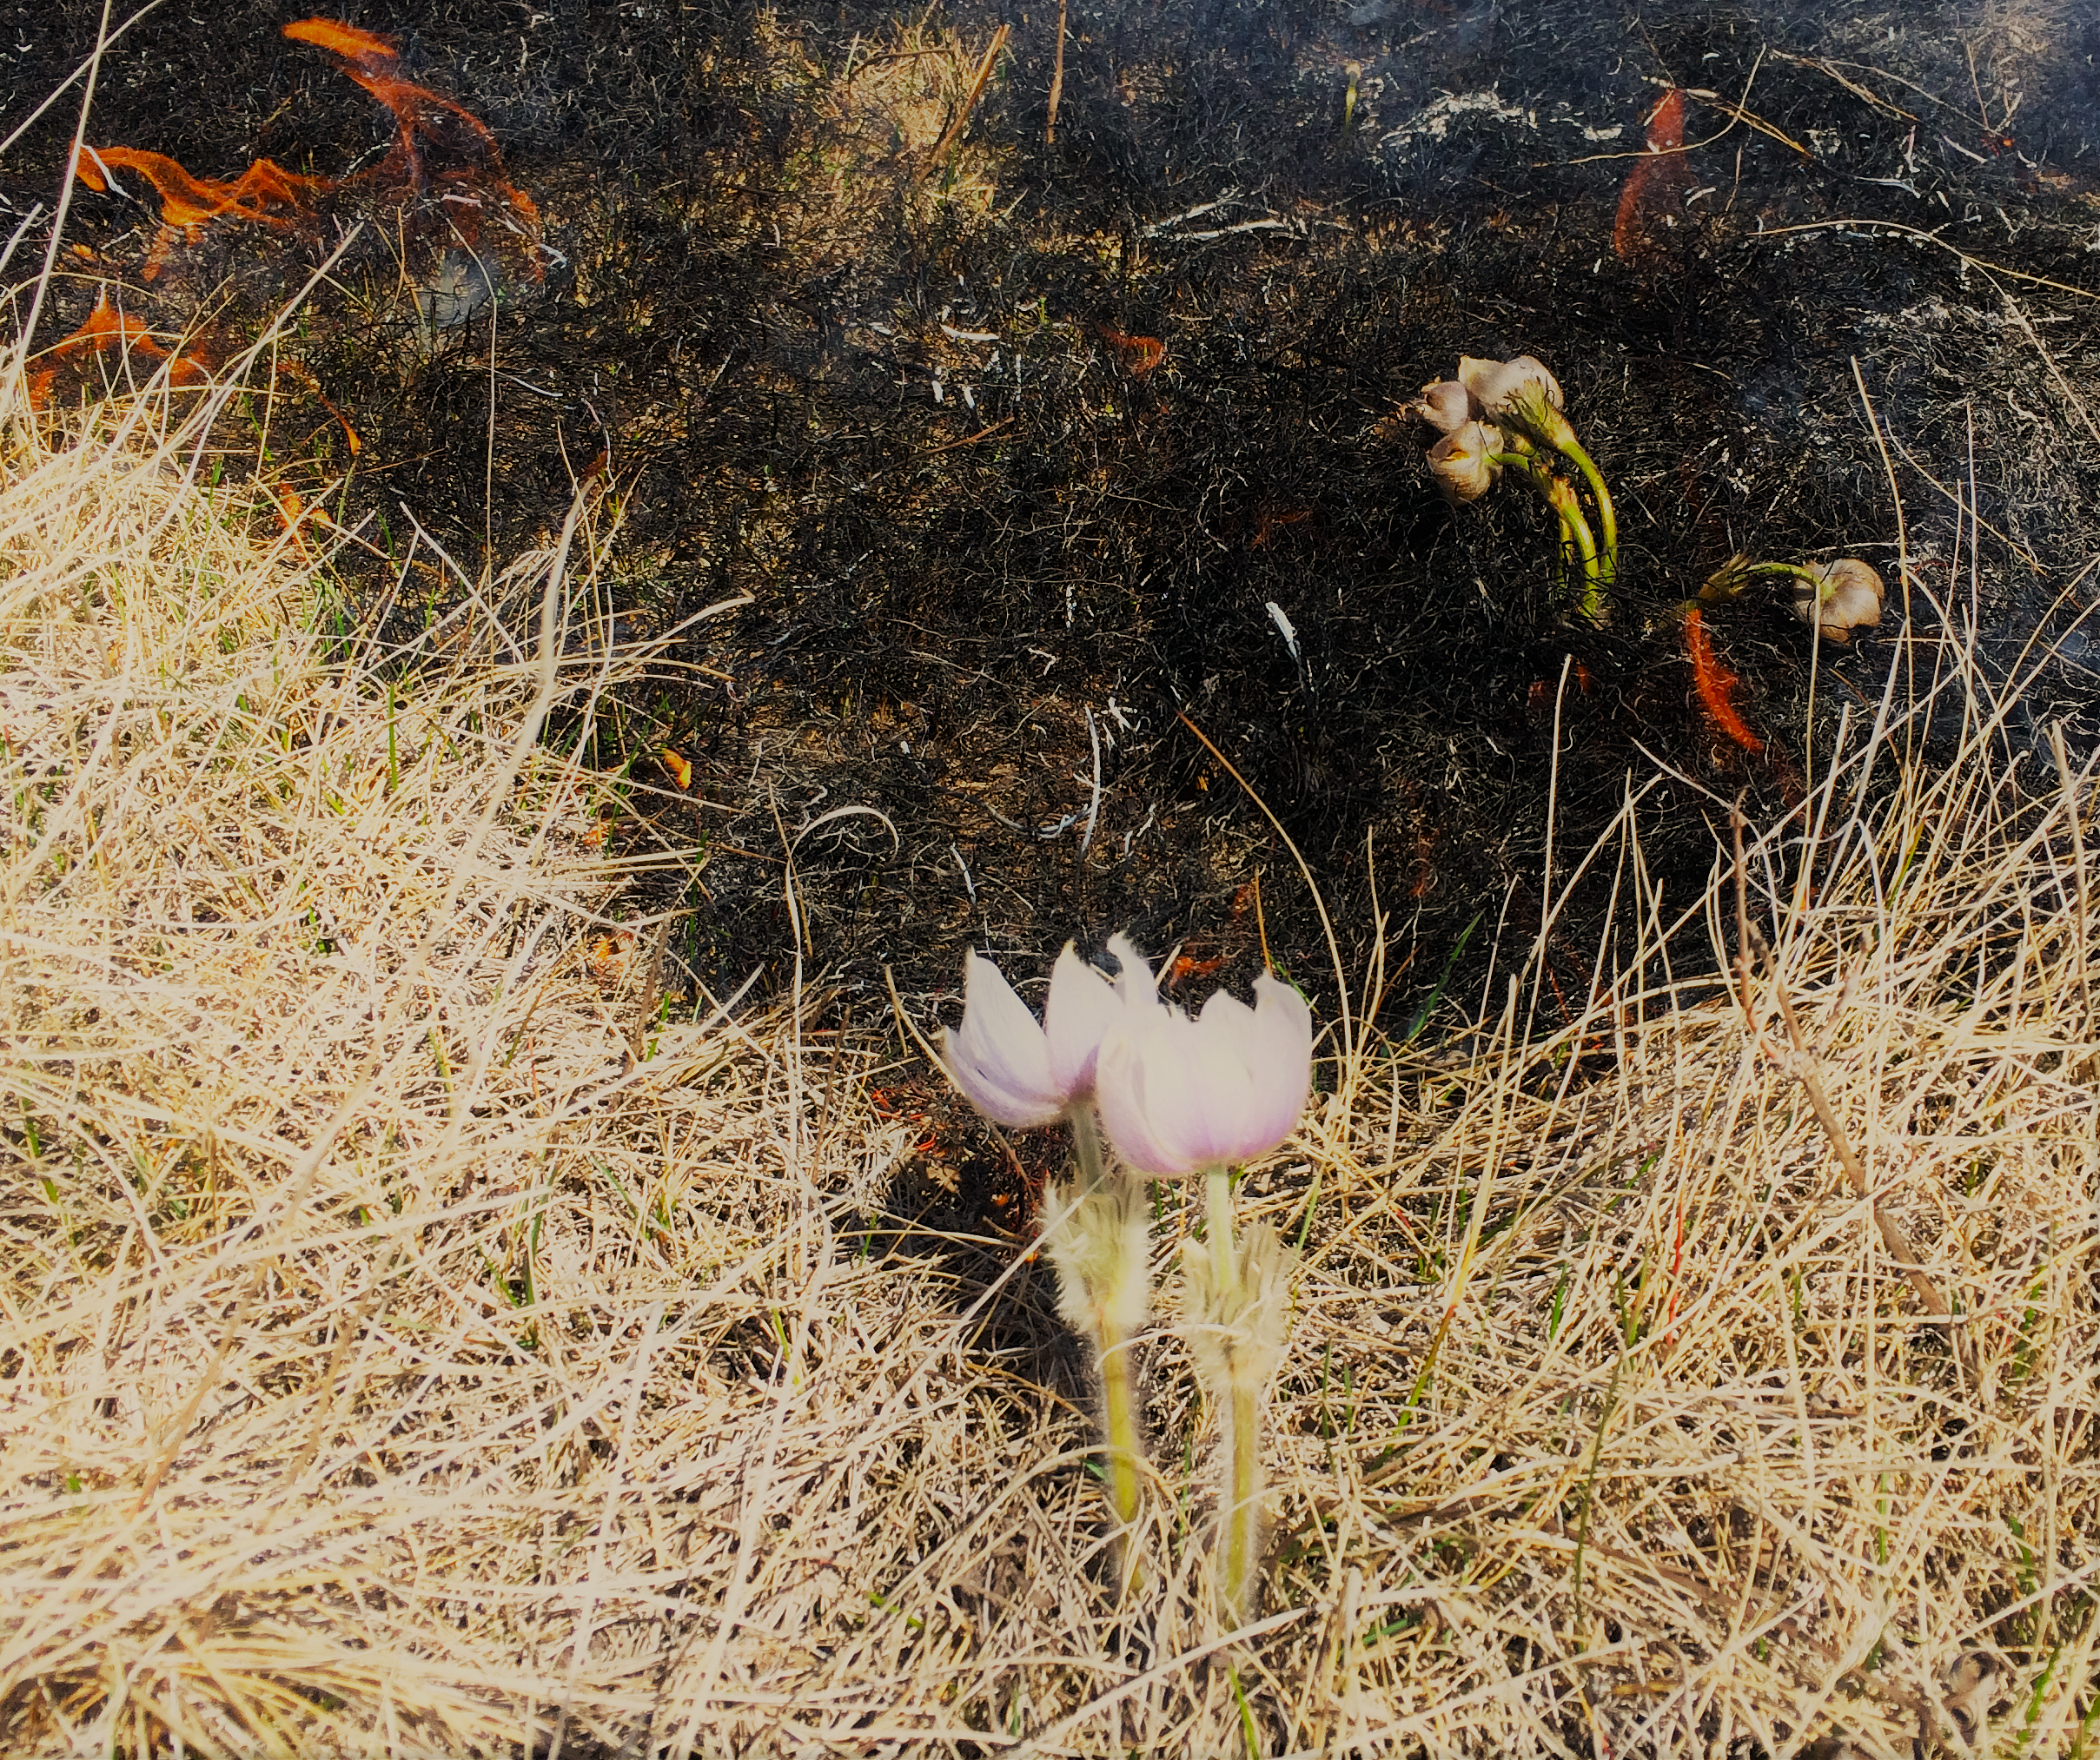
\includegraphics[width=1\linewidth]{figs/BurningPasqueFlowers} 
					\includegraphics[width=1\linewidth]{figs/MDubs2} 
					
				\end{figure}
			\end{center}
		\end{column}
	\end{columns}
\end{frame}

\begin{frame}{Thoughts, feedback, and discussion}
	\begin{center}
		\begin{figure}
			\includegraphics[width=1\linewidth]{figs/crew} 
			
		\end{figure}
	\end{center}
\end{frame}

\begin{frame}{Barriers to summer R\textsubscript{x} fire } 
	All opportunities and limitations fit within fire regime concept
	\begin{itemize}
		\item Biophysical 
		\item[] \emph{mostly, \alert{too wet}}
		\begin{itemize}
			\item High live moisture fuel content (\emph{photosynthesis})
			\item High dead moisture fuel content (\emph{humidity})
			\item Poor convection/smoke dispersal (\emph{humidity})
		\end{itemize}
		\item[]
		\item Social 
		\item[] \emph{mostly, \alert{too dry}}
		\begin{itemize}
			\item Local burn restrictions
			\item Control issues
		\end{itemize}
	\end{itemize}
\end{frame}

\section{Social barriers}

\begin{frame}{County-level burn restrictions}
	\begin{center}
		\begin{figure}
			\includegraphics[width=1\linewidth]{figs/FireDeclarations.png} 
		\end{figure}
	\end{center}
\end{frame}

\begin{frame}{County-level burn restrictions}
	\begin{center}
		\begin{figure}
			\includegraphics[width=1\linewidth]{figs/StutsmanBurnBan} 
		\end{figure}
	\end{center}
\end{frame}

\begin{frame}{Tying burn restrictions to real-time conditions}
	\begin{center}
		\begin{figure}
			\includegraphics[width=1\linewidth]{figs/StutsmanOrdinance} 
		\end{figure}
	\end{center}
\end{frame}


\begin{frame}{Fire regime management}
	Difficult to satisfy multiple socially-constructed parameters (e.g. \emph{force patterns})
	\begin{center}
		\begin{figure}
			\includegraphics[width=1\linewidth]{figs/venn} 
		\end{figure}
	\end{center}
\end{frame}

\begin{frame}{Fire regime management}
	\vspace{-3em}
	Better to tweak controllable components towards desired objectives (e.g. \emph{support processes})
	\begin{center}
		\begin{figure}
			\includegraphics[width=1\linewidth]{figs/levers} 
		\end{figure}
	\end{center}
\end{frame}
%
%\begin{frame}{Fire regime management}
%	Better to tweak controllable components towards desired objectives (e.g. \emph{support processes})
%	\begin{center}
%		\begin{figure}
%			\includegraphics[width=1\linewidth]{figs/levers} 
%		\end{figure}
%	\end{center}
%\alert{Great Plains are in a \textbf{fire deficit} and management is best focused on \textbf{burning new acres}}
%\end{frame}
%

%
%
%
%\begin{frame}{Mopping up} 
%
%\begin{columns}
%\begin{column}{0.55\textwidth}
%\begin{itemize}
%	\item Fight the deficit: Burn what you can, when you can, but try to add new acres
%	\item[]
%		\item Focus on fine-scale levers to accomplish objectives regardless of season
%	\item[]
%	\item Consider emphasis on burn completeness: \emph{defend desired refugia}
%\end{itemize}
%\end{column}
%\end{columns}
%\end{frame}
%


\end{document}
